\chapter{Electricidad y magnetismo como un único campo relativista}

Hemos estudiado cómo un campo electromagnético prescrito hace que se mueva una partícula cargada. La mitad pendiente del problema es el propio campo: cómo evolucionan los campos eléctrico y magnético, y cómo la carga y la corriente actúan como sus fuentes. Las ecuaciones de Maxwell responden a esas preguntas. Sin embargo, antes de escribirlas, conviene recuperar el problema físico que hizo inevitable su estructura relativista.

Este es un retroceso deliberado respecto del formalismo. El principio de acción volverá, pero todavía no. Empezar por otro lado permite ver por qué los campos eléctrico y magnético deben ser partes de un mismo objeto antes de derivar su dinámica a partir de una acción.

\section{El problema del primer párrafo de Einstein}

Durante una visita a Bélgica, una conversación sobre los primeros congresos Solvay llevó de nuevo al artículo de 1905 de Einstein, \emph{Sobre la electrodinámica de los cuerpos en movimiento}. Su primer párrafo expone la motivación con notable concisión. Un mismo fenómeno electromagnético recibe dos explicaciones aparentemente distintas en dos sistemas de referencia inerciales. Un observador atribuye el efecto al magnetismo; otro, a la electricidad. El movimiento observado coincide, así que las dos descripciones no pueden corresponder a dos fenómenos físicos distintos.

El artículo ya está a nuestro alcance con las herramientas desarrolladas en este curso. Aunque no se siga cada cálculo, vale la pena leer el párrafo inicial porque plantea la pregunta adecuada antes de presentar la respuesta: ¿cómo pueden cambiar las descripciones eléctrica y magnética sin que cambie el suceso físico?

\subsection{Una carga, un imán y dos descripciones}

Consideremos un campo magnético dirigido según \(y\) y una carga que se mueve a lo largo del eje \(x\). En el sistema de referencia del laboratorio el campo eléctrico es nulo, así que la fuerza es magnética: \begin{equation}
\mathbf F=q\,\mathbf v\times\mathbf B.
\end{equation}La fuerza apunta en la otra dirección transversal. Los ejes esquemáticos que se dibujan rápidamente en la pizarra no pretenden fijar todos los signos de la regla de la mano derecha; lo importante es que la fuerza es perpendicular tanto a \(\mathbf v\) como a \(\mathbf B\), y que invertir el signo de la carga invierte la fuerza.

\begin{classroomqa}\audiencequestion{En el dibujo, ¿la fuerza apunta hacia arriba o hacia abajo?}\lecturerresponse{Eso depende del signo de la carga. Una vez fijadas la orientación de los ejes y el signo de \(q\), la regla de la mano derecha determina la dirección. Para el argumento actual solo importa que haya una fuerza transversal. \lecturetimestamp{00:07:13}}\end{classroomqa}

Einstein describió un hilo conductor, no una partícula aislada. Los átomos forman una red aproximadamente fija, mientras que los portadores móviles de carga se desplazan por ella. A comienzos del siglo XX también era mucho más fácil observar una corriente en un hilo que la trayectoria de una sola partícula cargada libre. Aquí esa distinción no es esencial: un portador en movimiento dentro de un campo magnético experimenta la misma fuerza de Lorentz.

\begin{figure}[H]\centering
\includegraphics[width=\linewidth]{lecture_08_figure_01.png}\caption{La carga en movimiento, el campo magnético transversal y la geometría del imán usados para replantear el problema electrodinámico de Einstein.}\par\smallskip
\textit{Fotograma de la clase: 00:07:00.}\end{figure}

Ahora dejemos fijo el hilo, o la carga de prueba, y movamos el imán. La configuración magnética variable produce una fuerza electromotriz que, en el lenguaje local, es un campo eléctrico. Ese campo eléctrico ejerce una fuerza sobre la carga estacionaria en la misma dirección transversal. Por tanto, las dos descripciones son \begin{align}
\text{moving charge, fixed magnet:}\quad&
q\,\mathbf v\times\mathbf B,
\\
\text{fixed charge, moving magnet:}\quad&
q\,\mathbf E'.
\end{align}El movimiento relativo es el mismo. Así pues, una teoría de la relatividad debe explicar cómo un campo puramente magnético en un sistema de referencia adquiere una componente eléctrica en otro.

La electricidad y el magnetismo no son sustancias separadas. Son partes de un único campo relativista que dependen del sistema de referencia. Einstein aún no disponía de la notación moderna del tensor de campo, y en este párrafo no llamó transformaciones de Lorentz a los cambios de sistema de referencia necesarios. Aun así, la cuestión de cómo se transforma el campo ya está plenamente planteada.

\section{El tensor del campo electromagnético}

El objeto que puede reunir los datos eléctricos y magnéticos es el tensor antisimétrico \begin{equation}
F_{\mu\nu}
=
\partial_\mu A_\nu-\partial_\nu A_\mu.
\label{eq:field-tensor-definition}
\end{equation}Los índices griegos recorren los valores \(0,1,2,3\), con \(x^0=t\); los índices latinos recorren los tres valores espaciales. La antisimetría, \begin{equation}
F_{\mu\nu}=-F_{\nu\mu},
\end{equation}anula las entradas diagonales y deja seis componentes independientes. Estas son precisamente las tres componentes de \(\mathbf E\) y las tres de \(\mathbf B\).

Con la métrica de signatura mayoritaria positiva \begin{equation}
\eta_{\mu\nu}=\operatorname{diag}(-1,1,1,1),
\end{equation}y la convención heredada de la acción de la partícula cargada de la clase anterior, definimos \begin{align}
E_m&=F_{0m}
=\partial_0A_m-\partial_mA_0,
\label{eq:e-from-a}
\\
B_i&=(\boldsymbol\nabla\times\mathbf A)_i.
\label{eq:b-from-a}
\end{align}Al escribir la primera línea, en la clase se corrige un índice espacial. La relación correcta es la que aparece arriba: el índice espacial libre debe coincidir en ambos lados.

\begin{figure}[H]\centering
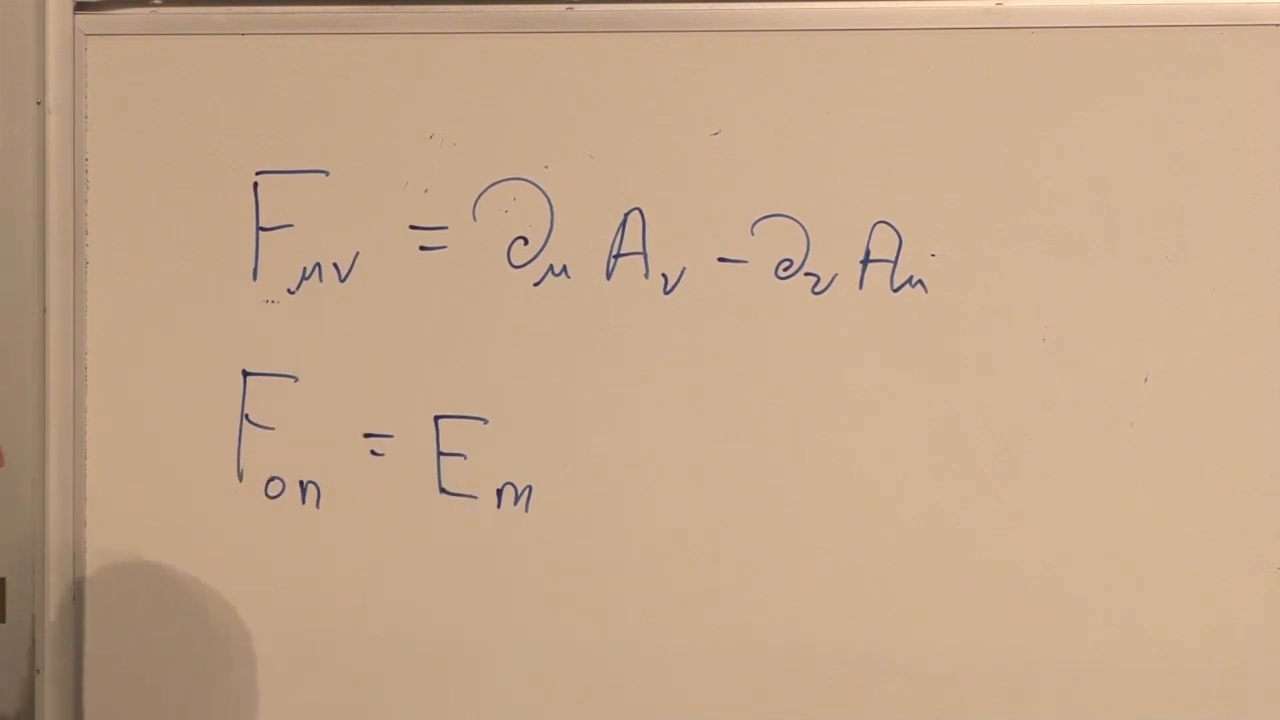
\includegraphics[width=\linewidth]{lecture_08_figure_02.png}\caption{La definición del tensor de campo y la componente mixta temporal--espacial identificada con el campo eléctrico.}\par\smallskip
\textit{Fotograma de la clase: 00:13:15.}\end{figure}

La relación magnética es la parte espacial de la misma definición. Por ejemplo, \begin{equation}
B_x
=
\partial_yA_z-\partial_zA_y
=
F_{yz},
\end{equation}; las otras dos componentes se obtienen mediante permutaciones cíclicas.

\begin{figure}[H]\centering
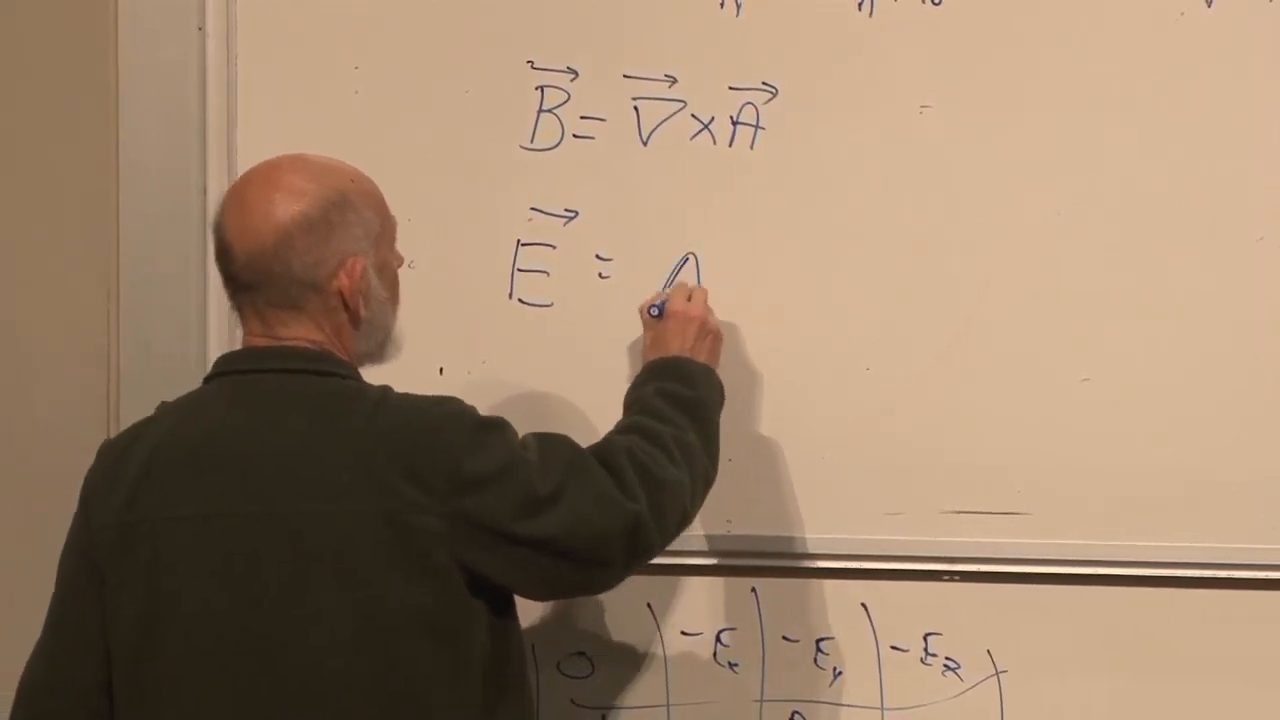
\includegraphics[width=\linewidth]{lecture_08_figure_03.png}\caption{Las fórmulas del potencial vector para el campo eléctrico y el rotacional del campo magnético, reunidas en la pizarra.}\par\smallskip
\textit{Fotograma de la clase: 00:14:00.}\end{figure}

\subsection{La matriz de componentes}

Sea el primer índice del tensor el que etiqueta las filas y el segundo el que etiqueta las columnas, ordenadas como \(0,x,y,z\). Entonces, \begin{equation}
F_{\mu\nu}
=
\begin{pmatrix}
0&E_x&E_y&E_z\\
-E_x&0&B_z&-B_y\\
-E_y&-B_z&0&B_x\\
-E_z&B_y&-B_x&0
\end{pmatrix}.
\label{eq:f-lower-matrix}
\end{equation}La arista temporal--espacial contiene \(\mathbf E\); el bloque espacial \(3\times3\) contiene \(\mathbf B\). El triángulo inferior no aporta información nueva, pues es el reflejo negativo del triángulo superior.

\begin{figure}[H]\centering
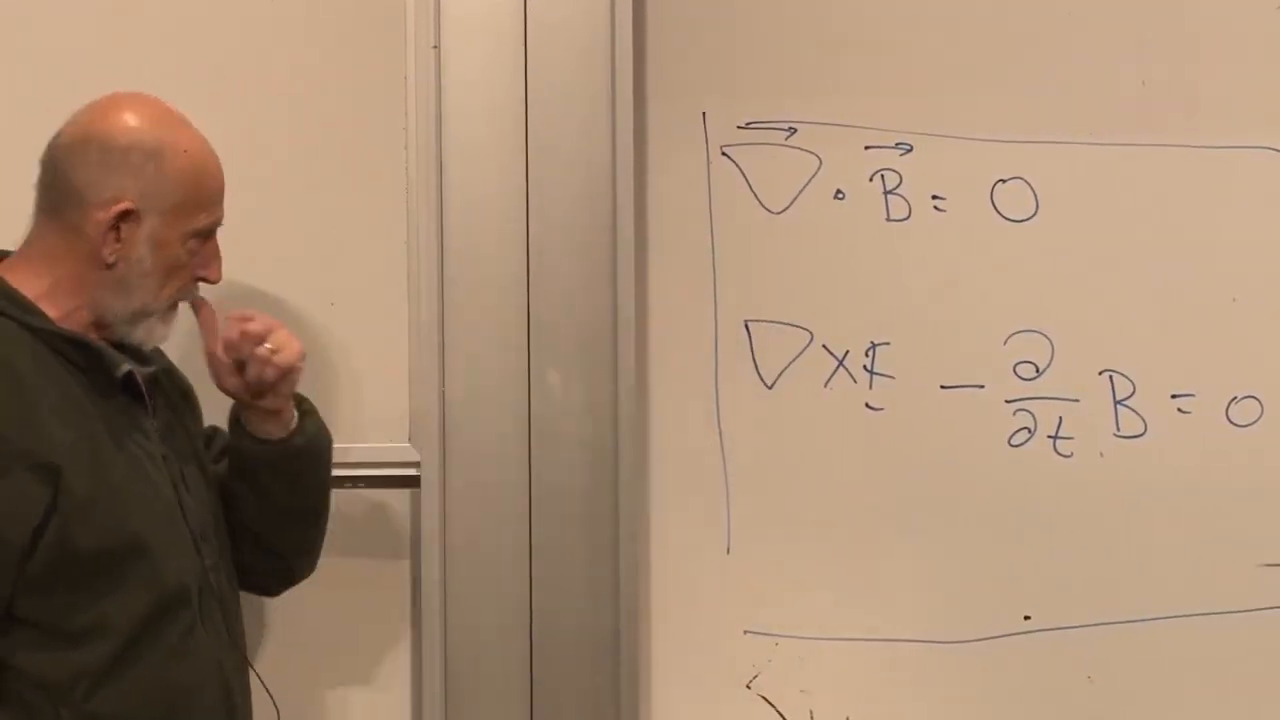
\includegraphics[width=\linewidth]{lecture_08_figure_04.png}\caption{El tensor electromagnético de índices abajo, completo, con su arista eléctrica y su bloque magnético espacial.}\par\smallskip
\textit{Fotograma de la clase: 00:17:15.}\end{figure}

Al subir ambos índices cambia el signo de cada entrada eléctrica, mientras que las entradas magnéticas permanecen iguales: \begin{equation}
F^{\mu\nu}
=
\begin{pmatrix}
0&-E_x&-E_y&-E_z\\
E_x&0&B_z&-B_y\\
E_y&-B_z&0&B_x\\
E_z&B_y&-B_x&0
\end{pmatrix}.
\label{eq:f-upper-matrix}
\end{equation}Una componente eléctrica tiene un índice temporal y, por tanto, recibe un signo menos. Una componente magnética tiene dos índices espaciales y no recibe ninguno.

\begin{classroomqa}\audiencequestion{¿Interpreto bien la matriz: las componentes magnéticas no tienen índice temporal?}\lecturerresponse{Sí. Ocupan el bloque puramente espacial. Las componentes eléctricas son precisamente las entradas mixtas temporal--espaciales de la primera fila y la primera columna. \lecturetimestamp{00:18:55}}\end{classroomqa}

\section{Transformación de un campo puramente magnético mediante un boost}

Consideremos un boost a lo largo de \(x\), con \(c=1\): \begin{align}
t'&=\gamma(t-vx),
&
x'&=\gamma(x-vt),
&
y'&=y,
&
z'&=z,
\end{align}donde \begin{equation}
\gamma=\frac{1}{\sqrt{1-v^2}}.
\end{equation}En forma matricial, \begin{equation}
x'^\mu
=
\Lambda^\mu{}_\nu x^\nu,
\qquad
\Lambda^\mu{}_\nu
=
\begin{pmatrix}
\gamma&-\gamma v&0&0\\
-\gamma v&\gamma&0&0\\
0&0&1&0\\
0&0&0&1
\end{pmatrix}.
\label{eq:x-boost}
\end{equation}

\begin{classroomqa}\audiencequestion{¿Falta un signo menos en la matriz del boost?}\lecturerresponse{Sí. Las entradas no diagonales temporal--espaciales llevan los signos menos exigidos por \(t'=\gamma(t-vx)\) y \(x'=\gamma(x-vt)\). La corrección se hace antes de usar la transformación del campo. \lecturetimestamp{00:23:50}}\end{classroomqa}

\begin{figure}[H]\centering
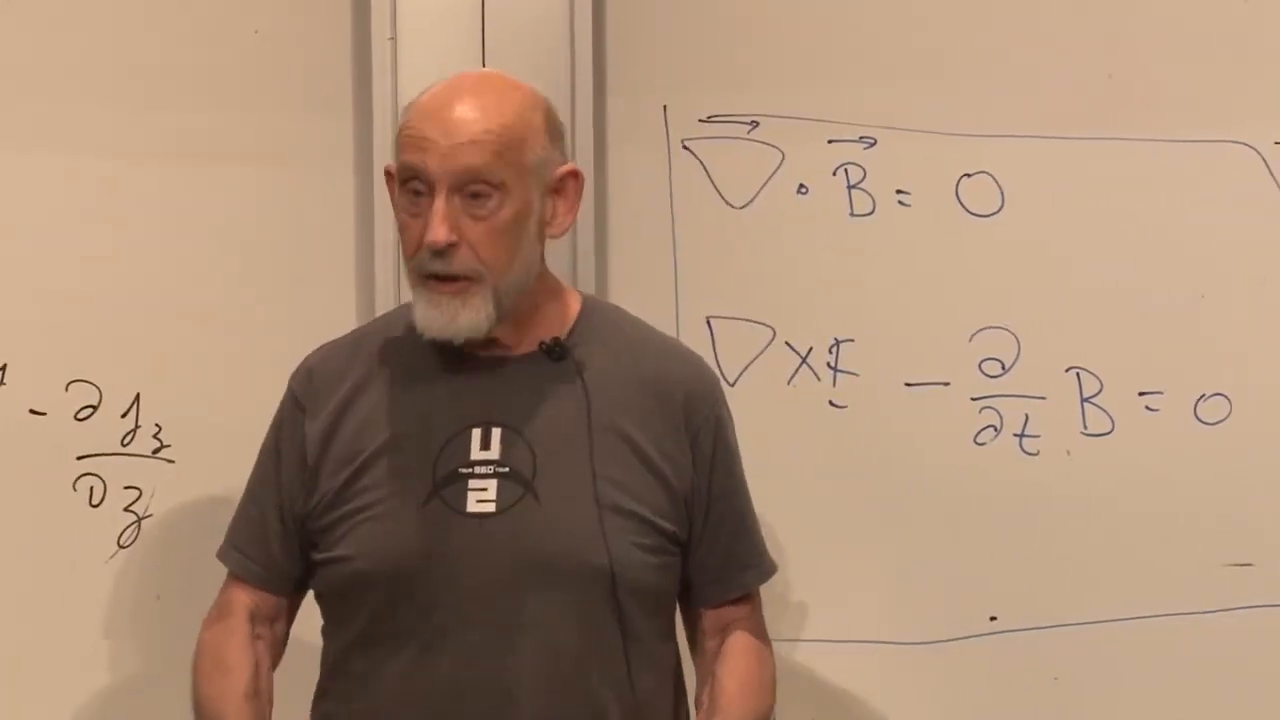
\includegraphics[width=\linewidth]{lecture_08_figure_05.png}\caption{La matriz corregida del boost de Lorentz para el movimiento a lo largo del eje \(x\).}\par\smallskip
\textit{Fotograma de la clase: 00:24:00.}\end{figure}

Cada índice tensorial contravariante se transforma como un índice contravariante de vector. Por tanto, \begin{equation}
F'^{\mu\nu}
=
\Lambda^\mu{}_\sigma
\Lambda^\nu{}_\tau
F^{\sigma\tau}.
\label{eq:f-boost-law}
\end{equation}Los índices repetidos \(\sigma\) y \(\tau\) son índices mudos. Para un tensor con más índices aparecería una matriz de transformación por cada índice.

\begin{figure}[H]\centering
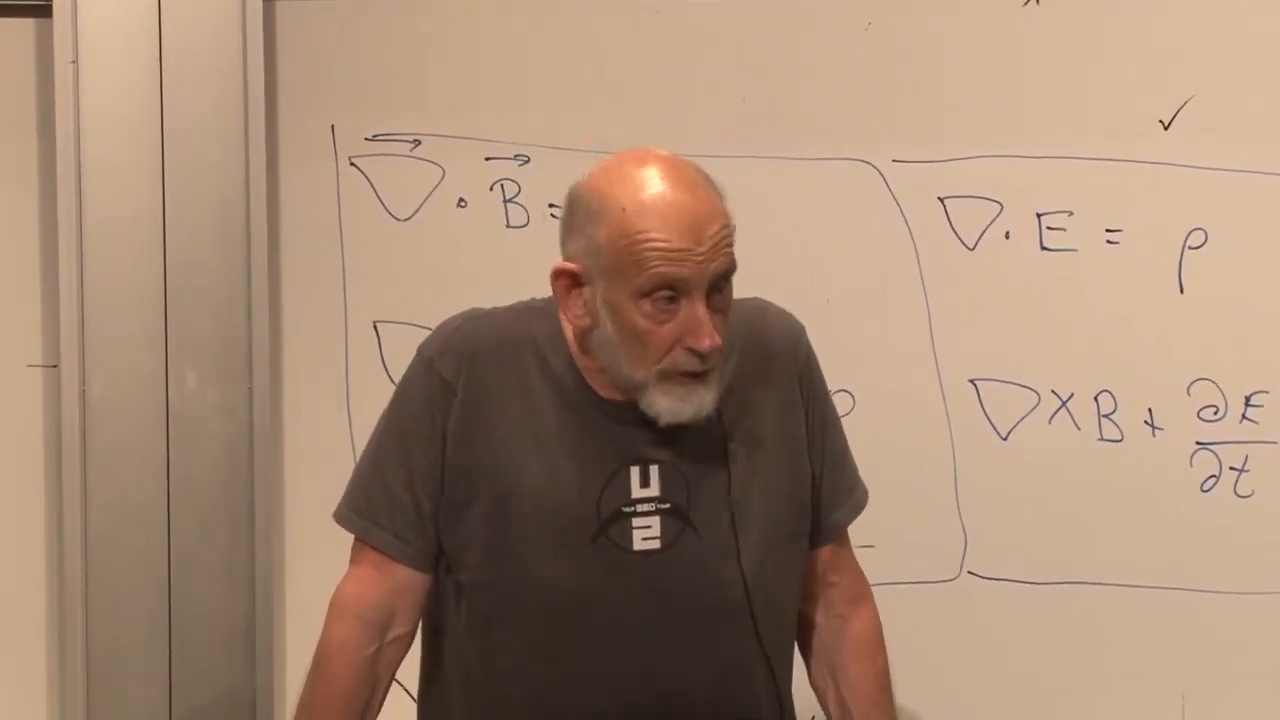
\includegraphics[width=\linewidth]{lecture_08_figure_06.png}\caption{La ley de transformación de Lorentz de un tensor de rango dos, con una matriz de boost para cada índice del tensor de campo.}\par\smallskip
\textit{Fotograma de la clase: 00:26:40.}\end{figure}

\subsection{La componente que se convierte en eléctrica}

Supongamos que en el sistema de referencia sin primas solo hay un campo magnético \(B_y\). Según las convenciones de la ecuación~\eqref{eq:f-upper-matrix}, la componente independiente pertinente es \begin{equation}
F^{xz}=-B_y.
\end{equation}Buscamos la componente mixta con primas \(F'^{0z}\), porque contiene la componente \(z\) del campo eléctrico en ese sistema. La ecuación \eqref{eq:f-boost-law} da \begin{align}
F'^{0z}
&=
\Lambda^0{}_\sigma
\Lambda^z{}_\tau F^{\sigma\tau}
\\
&=
\Lambda^0{}_x\Lambda^z{}_zF^{xz}
\\
&=
(-\gamma v)(1)(-B_y)
=
\gamma vB_y.
\end{align}Como en esta convención \(F'^{0z}=-E'_z\), \begin{equation}
E'_z=-\gamma vB_y.
\label{eq:boosted-electric-field}
\end{equation}El signo depende de las convenciones declaradas para los ejes y el campo; el resultado invariante del cálculo es \begin{equation}
\lvert E'_z\rvert
=
\gamma\lvert vB_y\rvert
\ne0.
\end{equation}La suma doble se reduce a un solo término porque el campo original tiene únicamente esta componente magnética independiente.

\begin{figure}[H]\centering
\includegraphics[width=\linewidth]{lecture_08_figure_07.png}\caption{La componente del tensor seleccionada después del boost, con el factor \(\gamma v\) que multiplica a la componente magnética original.}\par\smallskip
\textit{Fotograma de la clase: 00:32:30.}\end{figure}

Elijamos el sistema de referencia con primas de modo que se mueva junto con la carga. Entonces la carga está en reposo, de modo que no hay componente magnética \(q\,\mathbf v'\times\mathbf B'\) de la fuerza que experimenta. Sin embargo, la fuerza no desaparece: es \(q\mathbf E'\). La fuerza magnética que describe el observador del laboratorio y la fuerza eléctrica que describe el observador comóvil son dos descripciones del mismo suceso.

Esa es la respuesta al problema del primer párrafo de Einstein. La pregunta ocupó aproximadamente los primeros cuarenta minutos de esta clase; la broma histórica es que a Einstein le ocupó mucho más tiempo. El cálculo merece ese tiempo porque convierte en una componente explícita del tensor la afirmación de que los campos eléctrico y magnético se mezclan.

\section{Ecuaciones de Maxwell: identidades y dinámica}

Pasemos ahora de la fuerza sobre una carga a las ecuaciones de campo. Se derivarán a partir de una acción en la próxima clase. Aquí el propósito es, primero, enunciarlas, entender sus dos funciones lógicas distintas y escribir en forma covariante la mitad que se basa en identidades.

\begin{classroomqa}\audiencequestion{¿No habíamos derivado ya estas ecuaciones?}\lecturerresponse{Derivamos la ecuación de movimiento de una partícula cargada en un campo electromagnético prescrito. Las ecuaciones de Maxwell son ecuaciones de movimiento del propio campo, incluida la respuesta del campo a la carga y la corriente. \lecturetimestamp{00:35:10}}\end{classroomqa}

\begin{classroomqa}\audiencequestion{¿Cuántas ecuaciones de Maxwell hay?}\lecturerresponse{Hay ocho ecuaciones escalares para las componentes. La notación vectorial las agrupa como dos ecuaciones escalares y dos ecuaciones vectoriales de tres componentes, que convencionalmente se denominan las cuatro ecuaciones de Maxwell. \lecturetimestamp{00:35:24}}\end{classroomqa}

Seguimos usando unidades en las que \(c=1\) y las constantes habituales del vacío se han absorbido en las definiciones de carga y corriente. Cuatro de las ocho ecuaciones para las componentes se deducen de la definición \(F=dA\). Son identidades cinemáticas. Las otras cuatro son dinámicas y podrían cambiar si cambiara la acción del campo.

\subsection{Tres operaciones vectoriales elementales}

Para un campo vectorial tridimensional diferenciable \(\mathbf A\), \begin{align}
(\boldsymbol\nabla\times\mathbf A)_x
&=
\partial_yA_z-\partial_zA_y,
\\
\boldsymbol\nabla\cdot\mathbf A
&=
\partial_xA_x+\partial_yA_y+\partial_zA_z.
\end{align}Las componentes restantes del rotacional se obtienen mediante permutaciones cíclicas de \(x\to y\to z\to x\). Para un campo escalar \(s\), \begin{equation}
\boldsymbol\nabla s
=
(\partial_xs,\partial_ys,\partial_zs).
\end{equation}Así, el rotacional es un vector, la divergencia es un escalar y el gradiente es un vector.

\begin{classroomqa}\audiencequestion{¿Hace falta repasar por completo las definiciones de rotacional y divergencia?}\lecturerresponse{Las definiciones por componentes quedan anotadas, pero no hace falta desarrollar todas las demás componentes. Se obtienen ciclando las etiquetas de las coordenadas. \lecturetimestamp{00:37:32}}\end{classroomqa}

La conmutatividad de las derivadas parciales de funciones suaves implica dos identidades: \begin{align}
\boldsymbol\nabla\cdot
(\boldsymbol\nabla\times\mathbf A)
&=0,
\label{eq:div-curl}
\\
\boldsymbol\nabla\times
(\boldsymbol\nabla s)
&=\mathbf0.
\label{eq:curl-grad}
\end{align}

\begin{classroomqa}\audiencequestion{¿Debemos escribir la demostración completa por componentes de que la divergencia de un rotacional es nula?}\lecturerresponse{La clase decide que no. Al desarrollar las componentes aparecen pares como \(\partial_x\partial_yA_z\) y \(-\partial_y\partial_xA_z\), que se anulan porque se puede intercambiar el orden de las derivadas. \lecturetimestamp{00:40:13}}\end{classroomqa}

\begin{figure}[H]\centering
\includegraphics[width=\linewidth]{lecture_08_figure_08.png}\caption{Las identidades de la divergencia del rotacional y del rotacional del gradiente, usadas para obtener la mitad de las ecuaciones de Maxwell.}\par\smallskip
\textit{Fotograma de la clase: 00:41:40.}\end{figure}

\subsection{Ausencia de fuentes magnéticas a partir del potencial vector}

Al tomar la divergencia de la ecuación~\eqref{eq:b-from-a}, obtenemos \begin{equation}
\boldsymbol\nabla\cdot\mathbf B
=
\boldsymbol\nabla\cdot
(\boldsymbol\nabla\times\mathbf A)
=0.
\label{eq:div-b-zero}
\end{equation}No se ha usado ninguna ecuación de movimiento. El resultado se sigue únicamente de la descripción mediante potenciales y de la suavidad de las derivadas.

\begin{figure}[H]\centering
\includegraphics[width=\linewidth]{lecture_08_figure_09.png}\caption{La divergencia del campo magnético reducida a la divergencia de un rotacional.}\par\smallskip
\textit{Fotograma de la clase: 00:43:05.}\end{figure}

\begin{classroomqa}\audiencequestion{¿Cuál es la divergencia del campo eléctrico?}\lecturerresponse{En las unidades que estamos usando, es la densidad de carga eléctrica: \(\boldsymbol\nabla\cdot\mathbf E=\rho\). Una carga puntual es el ejemplo prototípico de líneas de campo eléctrico que se extienden desde una fuente. \lecturetimestamp{00:43:20}}\end{classroomqa}

A este nivel elemental, la ecuación~\eqref{eq:div-b-zero} afirma que no hay densidad de carga magnética. Un potencial vector suave y definido globalmente no puede producir una fuente de monopolos magnéticos. Más adelante habrá que matizar esta afirmación: los monopolos pueden describirse con potenciales definidos en parches que se solapan o con elecciones de gauge singulares. La clase deja ese refinamiento para después.

\subsection{La ecuación de Faraday a partir del potencial eléctrico}

La ecuación~\eqref{eq:e-from-a}, escrita con notación vectorial tridimensional, es \begin{equation}
\mathbf E
=
\frac{\partial\mathbf A}{\partial t}
-\boldsymbol\nabla A_0.
\label{eq:e-vector-potential}
\end{equation}Aunque \(A_0\) forma parte de un cuadrivector, es un escalar bajo las rotaciones espaciales ordinarias. Tomemos el rotacional: \begin{align}
\boldsymbol\nabla\times\mathbf E
&=
\boldsymbol\nabla\times
\frac{\partial\mathbf A}{\partial t}
-
\boldsymbol\nabla\times
(\boldsymbol\nabla A_0)
\\
&=
\frac{\partial}{\partial t}
(\boldsymbol\nabla\times\mathbf A)
\\
&=
\frac{\partial\mathbf B}{\partial t}.
\end{align}El rotacional espacial conmuta con la derivada temporal, mientras que el rotacional del gradiente se anula.

\begin{figure}[H]\centering
\includegraphics[width=\linewidth]{lecture_08_figure_10.png}\caption{El rotacional magnético, la fórmula del potencial eléctrico y el comienzo del cálculo del rotacional, reunidos en un estado completo de la pizarra.}\par\smallskip
\textit{Fotograma de la clase: 00:47:45.}\end{figure}

Por tanto, las cuatro ecuaciones homogéneas para las componentes son \begin{align}
\boldsymbol\nabla\cdot\mathbf B&=0,
\label{eq:homogeneous-div}
\\
\boldsymbol\nabla\times\mathbf E
-\frac{\partial\mathbf B}{\partial t}
&=\mathbf0.
\label{eq:homogeneous-curl}
\end{align}La primera es una ecuación escalar; la segunda, una ecuación vectorial de tres componentes.

\begin{figure}[H]\centering
\includegraphics[width=\linewidth]{lecture_08_figure_11.png}\caption{El par homogéneo de ecuaciones de Maxwell obtenido directamente de las definiciones mediante potenciales.}\par\smallskip
\textit{Fotograma de la clase: 00:48:45.}\end{figure}

\subsection{La mitad dinámica}

Las ecuaciones restantes son \begin{align}
\boldsymbol\nabla\cdot\mathbf E&=\rho,
\label{eq:gauss-electric}
\\
\boldsymbol\nabla\times\mathbf B
+\frac{\partial\mathbf E}{\partial t}
&=-\mathbf J.
\label{eq:ampere-maxwell}
\end{align}No se deducen de \(F=dA\). Describen cómo las fuentes crean y modifican el campo, y en la próxima clase se derivarán a partir de la acción electromagnética. El signo menos de la corriente queda fijado por las convenciones ya elegidas: \(F_{0i}=E_i\), \(F_{ij}=\epsilon_{ijk}B_k\) y \(\partial_\mu F^{\mu\nu}=J^\nu\). En la pizarra, al principio se coloca \(\mathbf J\) a la derecha sin ese signo menos; en la clase siguiente se advierte y corrige la incompatibilidad resultante con la conservación de la carga.

\begin{classroomqa}\audiencequestion{¿Qué tipo de magnitud aparece en el lado derecho de la ecuación del rotacional?}\lecturerresponse{El lado izquierdo es un vector tridimensional, así que el lado derecho también lo es: se trata de la densidad de corriente eléctrica \(\mathbf J\). El lado derecho de la ecuación de Gauss es la densidad escalar tridimensional de carga \(\rho\). \lecturetimestamp{00:50:36}}\end{classroomqa}

\begin{figure}[H]\centering
\includegraphics[width=\linewidth]{lecture_08_figure_12.png}\caption{Las cuatro ecuaciones de Maxwell, agrupadas en el par basado en identidades y el par dinámico con fuentes.}\par\smallskip
\textit{Fotograma de la clase: 00:50:40.}\end{figure}

\section{La carga y la corriente como flujo en el espacio-tiempo}

Ahora hay que dar un significado geométrico a los símbolos \(\rho\) y \(\mathbf J\). La densidad de carga es la carga por unidad de volumen; la densidad de corriente es la carga que atraviesa un área orientada por unidad de tiempo. La clase define ambas mediante líneas de universo para que luego su unión en un cuadrivector no parezca accidental.

\subsection{Un aparte en clase a propósito de la pizarra contigua}

Antes de dibujar esas líneas de universo, las ecuaciones visibles en el aula contigua dan pie a un breve aparte docente. Un curso próximo introduciría la mecánica cuántica a profesores de matemáticas que querían adquirir los conocimientos de base necesarios para estudiar teoría cuántica de campos y sus conexiones con las matemáticas modernas. El reto va en ambas direcciones: el físico debe explicitar hábitos físicos tácitos, mientras que el matemático debe aprender qué se pretende describir con las estructuras formales.

\begin{classroomqa}\audiencequestion{¿Quién podría encontrar frustrante esa tarea docente?}\lecturerresponse{Posiblemente ambas partes: los físicos al enseñar a un público que les resulta poco familiar, y los matemáticos al enfrentarse a los hábitos físicos que subyacen al formalismo. Aun así, se espera que la tarea sea divertida. La clase vuelve entonces a la carga y la corriente. \lecturetimestamp{00:53:20}}\end{classroomqa}

\subsection{Densidad de carga}

Dibujemos el tiempo en vertical y representemos las tres dimensiones espaciales restantes mediante las demás direcciones del dibujo. Las partículas cargadas trazan líneas de universo. En un instante fijo, coloquemos un pequeño cubo espacial de volumen \(\Delta V\) de modo que corte ese haz de líneas de universo, y sumemos las cargas de las partículas que contiene. La densidad de carga es \begin{equation}
\rho(t,\mathbf x)
=
\lim_{\Delta V\to0}
\frac{\Delta Q}{\Delta V}.
\label{eq:charge-density}
\end{equation}El cuadrado bidimensional de la pizarra representa un cubo tridimensional; la dimensión espacial que falta se omite solo porque no es posible dibujar cuatro dimensiones en una pizarra plana.

\begin{figure}[H]\centering
\includegraphics[width=\linewidth]{lecture_08_figure_13.png}\caption{Líneas de universo de partículas cargadas que atraviesan una pequeña celda espacial, con \(\rho=\Delta Q/\Delta V\).}\par\smallskip
\textit{Fotograma de la clase: 00:57:20.}\end{figure}

\subsection{Densidad de corriente}

Giremos la celda del espacio-tiempo de lado. Para definir \(J_x\), elijamos una pequeña ventana de área \(\Delta A_x\) en el plano \(yz\), perpendicular al eje \(x\). Contemos la carga neta que cruza desde el lado de \(x\) negativo hacia el lado de \(x\) positivo durante \(\Delta t\): \begin{equation}
J_x
=
\lim_{\Delta A_x,\Delta t\to0}
\frac{\Delta Q_x}{\Delta A_x\,\Delta t}.
\label{eq:jx-window}
\end{equation}La orientación determina el signo. Del mismo modo se definen \(J_y\) y \(J_z\) mediante ventanas perpendiculares a \(y\) y \(z\), respectivamente.

La pizarra refleja con honestidad las dificultades del dibujo: una ventana en el plano \(yz\) parece una ventana en el techo, no en la pared. Sencillamente hay más ejes pertinentes de los que se pueden mostrar a la vez. La definición invariante no ofrece ambigüedad, aunque el esquema sí.

\begin{classroomqa}\audiencequestion{¿La ventana del dibujo está en el techo?}\lecturerresponse{En la analogía de la habitación, sí. Lo que importa es que su plano sea perpendicular a la dirección \(x\). Un área \(yz\) mide la corriente dirigida según \(x\) que la atraviesa. \lecturetimestamp{00:59:38}}\end{classroomqa}

\begin{figure}[H]\centering
\includegraphics[width=\linewidth]{lecture_08_figure_14.png}\caption{Corriente de carga a través de una ventana transversal, con \(J_x=\Delta Q/(\Delta A\,\Delta t)\).}\par\smallskip
\textit{Fotograma de la clase: 01:01:40.}\end{figure}

\begin{figure}[H]\centering
\includegraphics[width=\linewidth]{lecture_08_figure_15.png}\caption{Las tres componentes de la corriente, definidas mediante el paso de carga a través de ventanas normales a los tres ejes espaciales.}\par\smallskip
\textit{Fotograma de la clase: 01:02:40.}\end{figure}

Las cuatro magnitudes tienen definiciones paralelas. Un volumen espacial en un instante es una hipersuperficie perpendicular al eje temporal, de modo que \(\rho\) es el flujo de carga a través de una ventana normal al tiempo. Las magnitudes \(J_i\) son flujos a través de ventanas normales a las direcciones espaciales.

\begin{classroomqa}\audiencequestion{¿Las cuatro cantidades son un flujo en la dirección temporal y tres flujos en las direcciones espaciales?}\lecturerresponse{Esa es precisamente la imagen útil. Un volumen espacial es una ventana perpendicular al eje temporal; las tres áreas transversales son ventanas perpendiculares a \(x\), \(y\) y \(z\). Sus cuatro flujos forman un conjunto. \lecturetimestamp{01:04:14}}\end{classroomqa}

Esto sugiere la cuatrocorriente contravariante \begin{equation}
J^\mu
=
(\rho,J_x,J_y,J_z).
\label{eq:four-current}
\end{equation}

\begin{classroomqa}\audiencequestion{¿Dónde interviene la métrica y esta corriente es covariante o contravariante?}\lecturerresponse{Tal como se ha definido aquí, \(\rho\) y las tres componentes \(J_i\) forman las componentes de \(J^\mu\), un cuadrivector con índice arriba, es decir, contravariante. La métrica le baja el índice cuando se necesita \(J_\mu\). La formulación covariante de Maxwell mostrará por qué es natural elegir los índices arriba. \lecturetimestamp{01:04:48}}\end{classroomqa}

\section{Intermedio durante el descanso: señales cerca de un agujero negro}

Durante el descanso previsto, las preguntas vuelven a una conversación anterior sobre agujeros negros. Aunque es una digresión de la electrodinámica, se trata de un intercambio sustancial en clase que ilustra la misma disciplina de separar las descripciones de distintos observadores.

\begin{classroomqa}\audiencequestion{Si un observador lejano ve que un objeto que cae se ralentiza cerca del horizonte, ¿debería parecer que el agujero negro está cubierto por todo lo que ha caído en él?}\lecturerresponse{En el tiempo coordenado de Schwarzschild, se observa que la caída clásica se aproxima asintóticamente al horizonte. Puede imaginarse la materia que va cayendo como capas sucesivas cada vez más comprimidas cerca del horizonte. Sin embargo, en la práctica la señal saliente tarda cada vez más en llegar, sufre un mayor corrimiento al rojo y se vuelve más tenue. La luz emitida a una frecuencia local ordinaria llega primero como luz visible, luego como infrarroja, microondas y ondas de radio, y cada fotón transporta menos energía. Ningún detector distante realista sigue viendo para siempre un objeto brillante e inmóvil: se desvanece hasta desaparecer en la oscuridad. \lecturetimestamp{01:06:11}}\end{classroomqa}

Para el observador que cae, tanto su reloj como la linterna que emite luz localmente siguen siendo normales. La descripción distante difiere porque la frecuencia y la tasa de llegada sufren un corrimiento al rojo. Con energía y ancho de banda finitos, hay efectivamente una última parte del mensaje que se puede resolver.

\begin{classroomqa}\audiencequestion{¿El objeto se aproxima asintóticamente al horizonte de sucesos?}\lecturerresponse{Esa es la descripción distante en coordenadas de Schwarzschild. Desde el punto de vista cuántico, también hay que distinguir la señal que se desvanece de la radiación de Hawking del agujero negro. A tiempos suficientemente tardíos, la débil señal corrida al rojo se pierde observacionalmente en el fondo de radiación propia del agujero negro. \lecturetimestamp{01:09:24}}\end{classroomqa}

\begin{classroomqa}\audiencequestion{¿Qué ocurre si la longitud de onda corrida al rojo crece más allá de la escala del universo observable?}\lecturerresponse{En la práctica, la señal se pierde mucho antes de llegar a ese límite. La clase presenta la estimación de orden de magnitud de Hawking: aproximadamente un cuanto típico por tiempo de cruce de la luz, \[
t_{\rm cross}\sim\frac{R_s}{c}.
\]En un agujero negro grande, esta radiación es extraordinariamente débil, y una señal de caída suficientemente corrida al rojo se vuelve indetectable mucho antes de alcanzar cualquier límite cosmológico para la longitud de onda. \lecturetimestamp{01:09:50}}\end{classroomqa}

\begin{classroomqa}\audiencequestion{¿La tasa de aproximadamente un cuanto por tiempo de cruce se mantiene constante durante toda la vida del agujero negro?}\lecturerresponse{No. Un agujero negro de Schwarzschild que se evapora se contrae, por lo que disminuye su tiempo de cruce y aumenta su temperatura de Hawking. Así, la emisión se acelera. La estimación dimensional en función del radio instantáneo sigue siendo útil, pero el radio no es constante. En consecuencia, la longitud de onda típica de Hawking se acorta a medida que avanza la evaporación. \lecturetimestamp{01:11:42}}\end{classroomqa}

Tras el descanso, ya sin la chaqueta, volvemos a \(\rho\) y \(\mathbf J\).

\section{Conservación local de la carga}

Es tentador enunciar la conservación de la carga solo como \begin{equation}
\frac{dQ_{\rm universe}}{dt}=0.
\end{equation}Ese enunciado es demasiado débil. La carga podría desaparecer de un laboratorio y reaparecer instantáneamente en Alfa Centauri, o más lejos, en el cúmulo de Coma, sin que cambiara la carga total. Una ley así tendría poca fuerza experimental.

El enunciado más fuerte es local: la carga dentro de una región solo puede cambiar si cruza la frontera de esa región. Coloquemos una caja pequeña alrededor de un punto. Si su carga aumenta, debe haber una corriente neta entrante por sus seis caras; si disminuye, debe haber una corriente neta saliente.

\subsection{Flujo a través de caras opuestas}

Consideremos las dos caras perpendiculares a \(x\). La contribución entrante en una cara se evalúa en un valor de \(x\); la contribución en la cara opuesta se evalúa a una distancia pequeña. Su diferencia, dividida por el ancho de la caja, tiende a \begin{equation}
-\partial_xJ_x.
\end{equation}El signo menos aparece porque se define que \(J_x\) positivo corresponde al flujo hacia valores crecientes de \(x\), mientras que un flujo saliente reduce la carga de la caja. Los pares de caras en las direcciones \(y\) y \(z\) contribuyen de manera similar con \(-\partial_yJ_y\) y \(-\partial_zJ_z\). Por tanto, \begin{equation}
\frac{\partial\rho}{\partial t}
=
-\partial_xJ_x-\partial_yJ_y-\partial_zJ_z
=
-\boldsymbol\nabla\cdot\mathbf J.
\end{equation}Equivalentemente, \begin{equation}
\boxed{
\frac{\partial\rho}{\partial t}
+\boldsymbol\nabla\cdot\mathbf J=0
}.
\label{eq:continuity}
\end{equation}

\begin{figure}[H]\centering
\includegraphics[width=\linewidth]{lecture_08_figure_16.png}\caption{La ley local de balance \(\dot\rho=-\boldsymbol\nabla\cdot\mathbf J\), junto con la pequeña caja cuyas corrientes de frontera la producen.}\par\smallskip
\textit{Fotograma de la clase: 01:20:45.}\end{figure}

Esto se llama convencionalmente ecuación de continuidad. En la clase se prefiere el nombre de \emph{conservación local}: «continuidad» puede sugerir una hipótesis de suavidad matemática, mientras que el contenido físico es que la carga no puede desaparecer aquí y reaparecer allí sin que haya una corriente entre ambos puntos.

\subsection{Por qué Maxwell necesitó la corriente de desplazamiento}

La ecuación~\eqref{eq:continuity} no es una adición independiente a las ecuaciones de Maxwell. Derivemos respecto del tiempo la ley de Gauss y tomemos la divergencia de la ley de Ampère--Maxwell:
\begin{align}
\frac{\partial\rho}{\partial t}
&=
\boldsymbol\nabla\cdot
\frac{\partial\mathbf E}{\partial t},
\\
-\boldsymbol\nabla\cdot\mathbf J
&=
\boldsymbol\nabla\cdot
(\boldsymbol\nabla\times\mathbf B)
+
\boldsymbol\nabla\cdot
\frac{\partial\mathbf E}{\partial t}
\\
&=
\boldsymbol\nabla\cdot
\frac{\partial\mathbf E}{\partial t}.
\end{align}
Por tanto, los dos miembros de la izquierda son iguales, lo que da
\(\partial_t\rho=-\boldsymbol\nabla\cdot\mathbf J\), exactamente la ecuación~\eqref{eq:continuity}. Lo esencial desde el punto de vista estructural es que la derivada temporal de \(\mathbf E\), el término de corriente de desplazamiento, es imprescindible para que la relación de divergencia sea compatible con la conservación de la carga.

\begin{classroomqa}
\audiencequestion{No hemos mostrado de dónde vienen las dos ecuaciones de Maxwell con fuentes, ¿verdad?}
\lecturerresponse{No. Son el objetivo dinámico y las derivaremos de la acción en la próxima clase. La ley magnetostática del rotacional se conocía antes de Maxwell; la adición crucial de Maxwell, dependiente del tiempo, fue la corriente de desplazamiento. Su presencia hace que la ecuación de campo sea compatible con la conservación local de la carga. \lecturetimestamp{01:23:15}}
\end{classroomqa}

En la clase se deja como ejercicio el cálculo detallado de la divergencia, pero su conclusión no es opcional: las ecuaciones de Maxwell exigen la conservación de la carga.

\section{La cuatricorriente y su divergencia}

Escribamos la ecuación~\eqref{eq:continuity} por componentes:
\begin{equation}
\frac{\partial\rho}{\partial t}
+
\frac{\partial J_x}{\partial x}
+
\frac{\partial J_y}{\partial y}
+
\frac{\partial J_z}{\partial z}
=0.
\label{eq:continuity-components}
\end{equation}

\begin{figure}[H]\centering
\includegraphics[width=\linewidth]{lecture_08_figure_17.png}\caption{Conservación local de la carga, desarrollada en una derivada temporal y tres derivadas espaciales.}\par\smallskip
\textit{Marco de la clase: 01:25:40.}\end{figure}

Con \(J^\mu\) definido por la ecuación~\eqref{eq:four-current}, los cuatro términos forman una sola contracción:
\begin{equation}
\boxed{\partial_\mu J^\mu=0}.
\label{eq:four-current-conservation}
\end{equation}
El índice inferior de \(\partial_\mu\) se contrae con el índice superior de \(J^\mu\), de modo que el resultado es un escalar de Lorentz. La construcción geométrica con ventanas ya sugería esta ley de transformación: \(\rho\) y las tres componentes de la corriente son cuatro orientaciones de un mismo flujo de carga.

\begin{figure}[H]\centering
\includegraphics[width=\linewidth]{lecture_08_figure_18.png}\caption{Las componentes \((\rho,J_x,J_y,J_z)\) reunidas en \(J^\mu\) y contraídas con el gradiente de cuatro dimensiones.}\par\smallskip
\textit{Marco de la clase: 01:27:10.}\end{figure}

\begin{classroomqa}
\audiencequestion{¿Cuándo pasó la derivada temporal de \(\rho\) a ser una derivada parcial?}
\lecturerresponse{Desde el principio era una derivada parcial. Mantenemos fija la caja espacial y preguntamos cómo cambia su densidad de carga al transcurrir el tiempo. No seguimos una trayectoria en movimiento, así que \(\dot\rho\) significa aquí \(\partial\rho/\partial t\) a \(x,y,z\) fijos.
\lecturetimestamp{01:28:20}}
\end{classroomqa}

\section{Las ecuaciones homogéneas en forma covariante}

Ya tenemos los objetos necesarios:
\begin{itemize}
\item \(\mathbf E\) y \(\mathbf B\) son las seis componentes independientes del tensor antisimétrico \(F_{\mu\nu}\);
\item \(\rho\) y \(\mathbf J\) son las cuatro componentes de \(J^\mu\);
\item la conservación local es la ecuación escalar \(\partial_\mu J^\mu=0\).
\end{itemize}
La tarea que queda para esta clase es escribir el par homogéneo de ecuaciones de Maxwell, las ecuaciones~\eqref{eq:homogeneous-div} y \eqref{eq:homogeneous-curl}, como una sola ecuación tensorial.

\subsection{La derivada cíclica}

La respuesta es
\begin{equation}
\boxed{
\partial_\sigma F_{\nu\tau}
+
\partial_\nu F_{\tau\sigma}
+
\partial_\tau F_{\sigma\nu}
=0
}.
\label{eq:bianchi}
\end{equation}
Los tres términos asignan cíclicamente el índice de derivación y los dos índices del tensor de campo. A menudo se abrevia como
\begin{equation}
\partial_{[\sigma}F_{\nu\tau]}=0,
\end{equation}
donde los corchetes indican antisimetrización.

\begin{figure}[H]\centering
\includegraphics[width=\linewidth]{lecture_08_figure_19.png}\caption{La ecuación cíclica de tres índices que reúne las ecuaciones homogéneas de Maxwell.}\par\smallskip
\textit{Marco de la clase: 01:33:20.}\end{figure}

\subsection{Los tres índices espaciales}

Tomemos
\begin{equation}
(\sigma,\nu,\tau)=(x,y,z).
\end{equation}
Entonces
\begin{align}
0
&=
\partial_xF_{yz}
+
\partial_yF_{zx}
+
\partial_zF_{xy}
\\
&=
\partial_xB_x+\partial_yB_y+\partial_zB_z
\\
&=
\boldsymbol\nabla\cdot\mathbf B.
\end{align}
Así pues, la componente con todos los índices espaciales de la ecuación~\eqref{eq:bianchi} expresa precisamente que la divergencia magnética es nula.

\begin{figure}[H]\centering
\includegraphics[width=\linewidth]{lecture_08_figure_20.png}\caption{La componente con todos los índices espaciales de la identidad cíclica se reduce a \(\partial_xB_x+\partial_yB_y+\partial_zB_z=0\).}\par\smallskip
\textit{Marco de la clase: 01:35:30.}\end{figure}

\subsection{Un índice temporal}

Elijamos, por ejemplo,
\begin{equation}
(\sigma,\nu,\tau)=(y,x,0).
\end{equation}
Entonces, la ecuación~\eqref{eq:bianchi} combina dos derivadas espaciales de componentes eléctricas con una derivada temporal de una componente magnética:
\begin{equation}
\partial_yF_{x0}
+
\partial_xF_{0y}
+
\partial_0F_{yx}
=0.
\end{equation}
Usando la matriz de la ecuación~\eqref{eq:f-lower-matrix}, esta es una componente de
\begin{equation}
\boldsymbol\nabla\times\mathbf E
-\frac{\partial\mathbf B}{\partial t}
=\mathbf0,
\end{equation}
cuyos signos relativos quedan fijados por la antisimetría. Al elegir los otros pares de índices espaciales se obtienen las otras dos componentes del rotacional.

\begin{figure}[H]\centering
\includegraphics[width=\linewidth]{lecture_08_figure_21.png}\caption{Comprobación para una combinación de un índice temporal y dos espaciales, que produce una componente de la ecuación de Faraday.}\par\smallskip
\textit{Marco de la clase: 01:38:20.}\end{figure}

También hay una demostración directa. Sustituyamos la ecuación~\eqref{eq:field-tensor-definition} en la ecuación~\eqref{eq:bianchi}. Aparecen seis términos con derivadas segundas, que se cancelan por pares porque las derivadas parciales conmutan. Esta es la versión en cuatro dimensiones de las identidades de la divergencia del rotacional y el rotacional del gradiente.

\begin{classroomqa}
\audiencequestion{¿Hay una \(h\) en el nombre de Bianchi?}
\lecturerresponse{Sí. La ecuación cíclica es la identidad de Bianchi electromagnética, un caso particular de una identidad geométrica que también aparece en la relatividad general. Dejaremos para más adelante su interpretación geométrica más profunda.
\lecturetimestamp{01:40:28}}
\end{classroomqa}

\subsection{Por qué sesenta y cuatro componentes escritas representan solo cuatro ecuaciones}

Tres índices, cada uno con cuatro valores posibles, parecen dar lugar a \(4^3=64\) ecuaciones. La antisimetría elimina la redundancia:
\begin{itemize}
\item si dos índices coinciden, la expresión cíclica se anula idénticamente;
\item si los tres índices son distintos, las permutaciones reproducen la misma ecuación salvo por el signo;
\item en cuatro dimensiones solo hay \(\binom{4}{3}=4\) ternas no ordenadas de índices distintos.
\end{itemize}
Hay \(24\) ternas ordenadas con todos los índices distintos, agrupadas en cuatro conjuntos de seis permutaciones. Las \(40\) ternas ordenadas restantes se anulan. Las cuatro ecuaciones independientes son una ecuación para la divergencia magnética y las tres componentes de la ecuación de Faraday.

\begin{classroomqa}
\audiencequestion{El tensor de campo tiene seis componentes independientes, pero la expresión de tres índices parece contener sesenta y cuatro ecuaciones. ¿Por qué solo quedan cuatro?}
\lecturerresponse{Los índices repetidos dan cero, mientras que las permutaciones de tres índices distintos repiten la misma relación salvo por el signo. Así pues, las aparentemente sesenta y cuatro componentes se reducen a cuatro ecuaciones independientes.
\lecturetimestamp{01:41:58}}
\end{classroomqa}

La ecuación~\eqref{eq:bianchi} es manifiestamente tensorial y, por tanto, covariante de Lorentz. En la descripción con un potencial único y suave, también indica que no hay ni densidad de carga magnética ni corriente magnética. El par dinámico con fuentes queda justo en el punto al que llegó la clase: su ecuación covariante y su derivación a partir de la acción corresponden a la próxima sesión.

\section{Dualidad y la cuestión del monopolo}

Las preguntas finales vuelven a la aparente asimetría entre las fuentes eléctricas y magnéticas. En el espacio vacío, las ecuaciones de Maxwell admiten la rotación de dualidad eléctrica--magnética
\begin{equation}
\mathbf E\longrightarrow\mathbf B,
\qquad
\mathbf B\longrightarrow-\mathbf E.
\label{eq:duality-quarter-turn}
\end{equation}
Se trata de un giro de noventa grados en un plano abstracto cuyos ejes son \(\mathbf E\) y \(\mathbf B\), no de una reflexión que simplemente intercambia sus nombres. Si están presentes tanto fuentes eléctricas como magnéticas, las cuatricorrientes eléctrica y magnética deben rotar al mismo tiempo.

\begin{figure}[H]\centering
\includegraphics[width=\linewidth]{lecture_08_figure_22.png}\caption{Imagen final de la dualidad eléctrica--magnética: un cuarto de giro en el plano \(E\)-\(B\), en vez de un simple intercambio.}\par\smallskip
\textit{Marco de la clase: 01:45:00.}\end{figure}

\begin{classroomqa}
\audiencequestion{Si las ecuaciones sin fuentes son duales bajo el intercambio de los campos eléctrico y magnético, ¿por qué las componentes eléctricas son entradas temporal--espaciales, mientras que las magnéticas son entradas espacio--espaciales?}
\lecturerresponse{La distinción depende del marco de referencia dentro de \(F_{\mu\nu}\), y las ecuaciones sin fuentes admiten una rotación de dualidad. La operación correcta es \(\mathbf E\to\mathbf B\) y \(\mathbf B\to-\mathbf E\), y las corrientes de las fuentes rotan de forma análoga si se incluye la carga magnética. Un intercambio directo no recoge el signo necesario. \lecturetimestamp{01:43:25}}
\end{classroomqa}

\begin{classroomqa}
\audiencequestion{¿La descripción tensorial tan limpia vuelve carente de sentido al monopolo magnético?}
\lecturerresponse{No. Significa que un monopolo no puede representarse mediante un único potencial vectorial suave en todo el espacio. En su lugar, el potencial debe definirse por parches, hacerse singular de una forma dependiente del gauge o reemplazarse por una descripción dual equivalente. No se había observado ningún monopolo magnético elemental, y la clase promete volver a cómo encajan los monopolos en el formalismo, en vez de forzar la cuestión al final de la noche.
\lecturetimestamp{01:45:50}}
\end{classroomqa}

La clase termina, por tanto, en una frontera precisa. La relatividad ha explicado por qué se mezclan los campos eléctrico y magnético. Las definiciones mediante potenciales han proporcionado las ecuaciones homogéneas de Maxwell y su forma de Bianchi. El flujo de carga se ha convertido en la cuatricorriente, y la conservación local se ha expresado como \(\partial_\mu J^\mu=0\). Lo que queda es la dinámica: la acción electromagnética y la ecuación covariante de campo con fuentes.
